\begin{figure}[ht]
\begin{center}
   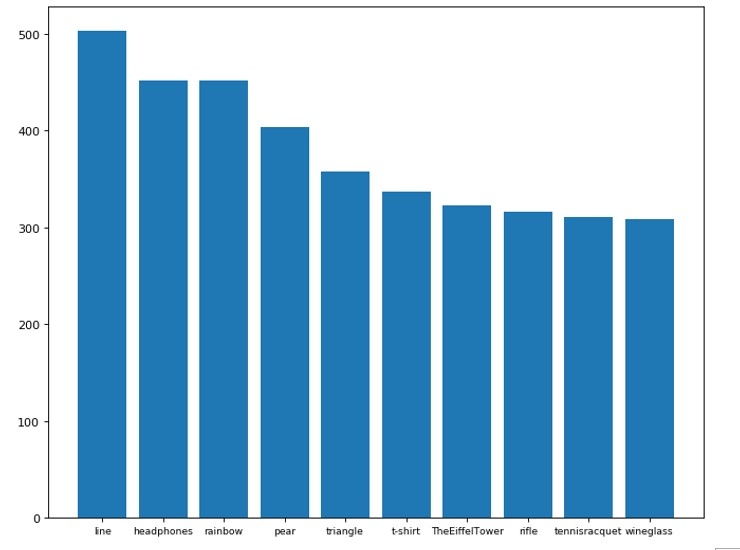
\includegraphics[width=1\linewidth]{figures/top_category.jpg}
\end{center}
   \caption{Top 10 categories with most similar drawing styles among all clusters}
\label{fig:top_category}
\end{figure}


\begin{figure}[ht]
\begin{center}
   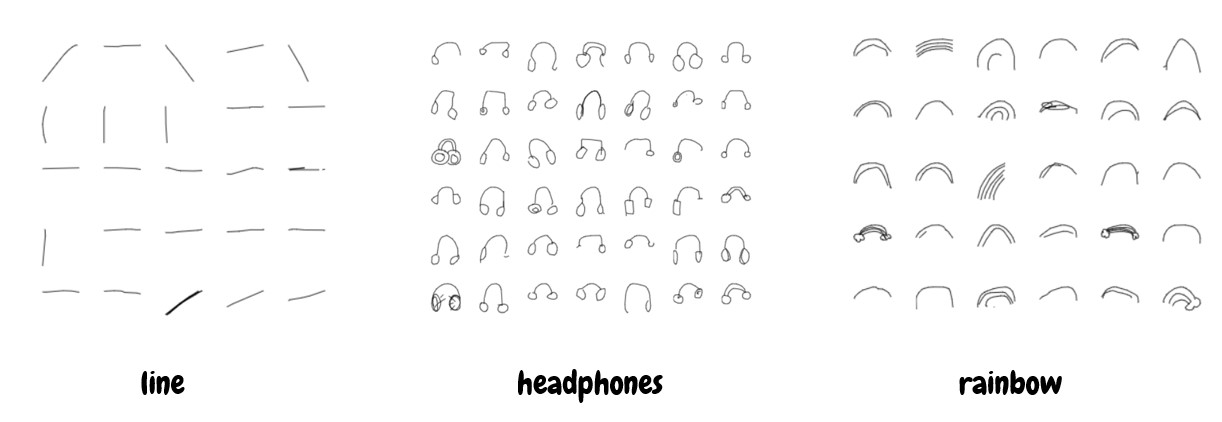
\includegraphics[width=1\linewidth]{figures/1.jpg}
\end{center}
   \caption{Examples of doodles in the top categories }
\label{fig:1}
\end{figure}


\begin{figure}[ht]
\begin{center}
   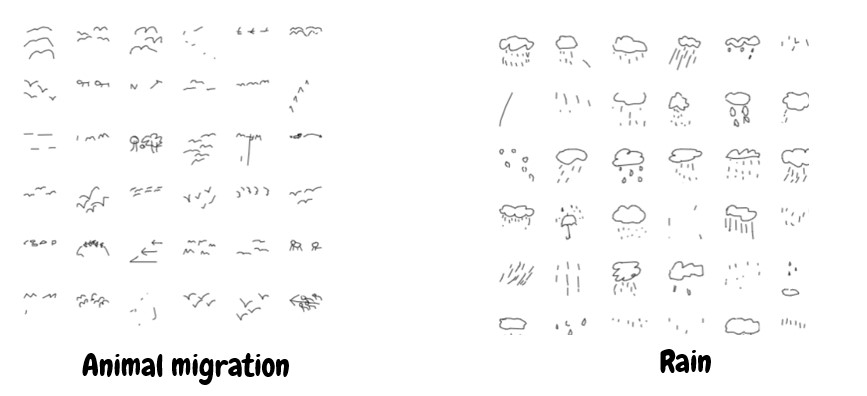
\includegraphics[width=1\linewidth]{figures/2.jpg}
\end{center}
   \caption{An examples of drawings with abstract category }
\label{fig:2}
\end{figure}

\begin{figure}[ht]
\begin{center}
   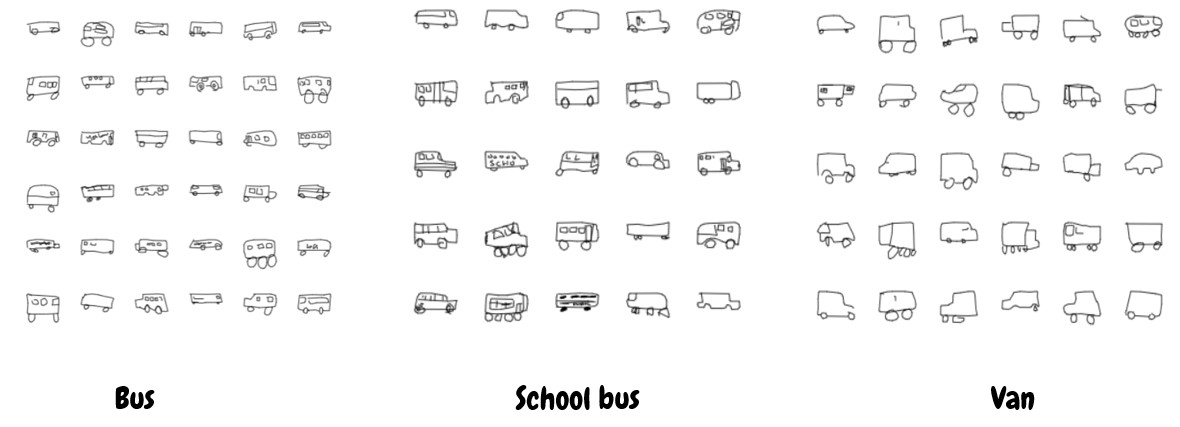
\includegraphics[width=1\linewidth]{figures/3.jpg}
\end{center}
   \caption{"Bus," "School Bus," and "Van" are in the same group}
\label{fig:3}
\end{figure}


\begin{figure}[ht]
\begin{center}
   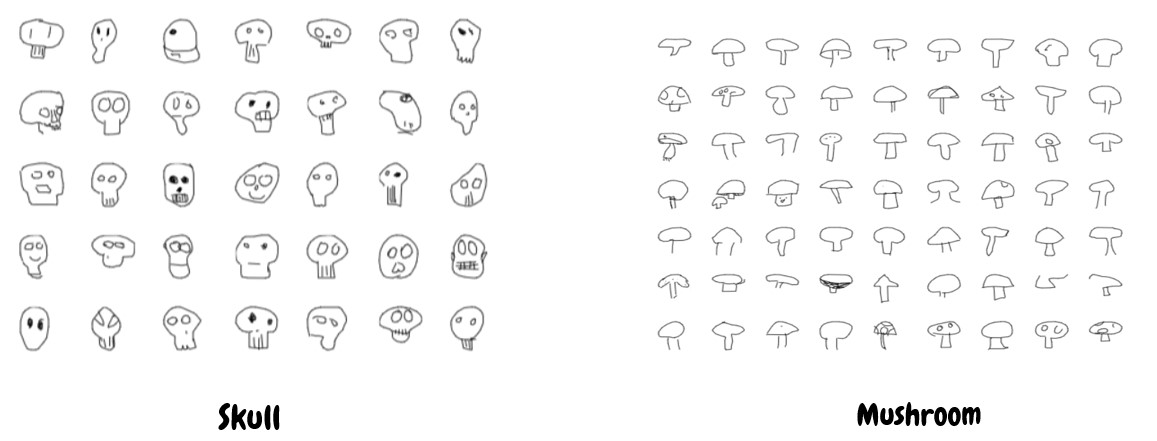
\includegraphics[width=1\linewidth]{figures/4.jpg}
\end{center}
   \caption{"Skull" and "Mushroom" are regarded as a same group}
\label{fig:4}
\end{figure}


\begin{figure}[ht]
\begin{center}
   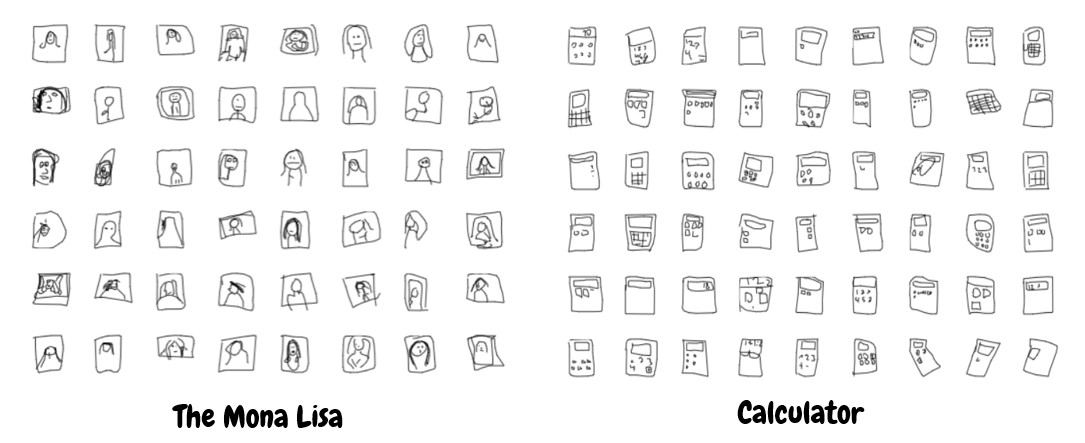
\includegraphics[width=1\linewidth]{figures/5.jpg}
\end{center}
   \caption{"The Mona Lisa" and "Calendar" are in a same cluster}
\label{fig:5}
\end{figure}

\begin{figure}[ht]
\begin{center}
   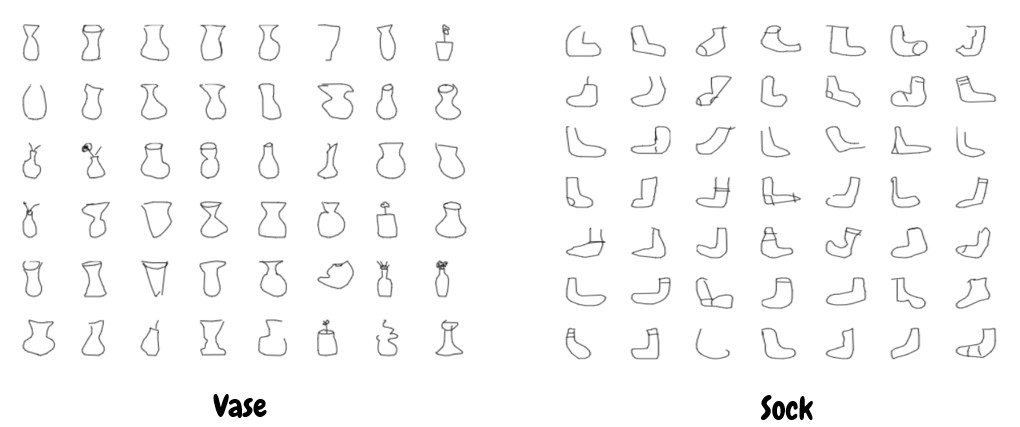
\includegraphics[width=1\linewidth]{figures/6.jpg}
\end{center}
   \caption{"Vase" and "Sock" are in a same cluster}
\label{fig:6}
\end{figure}